\documentclass[crop,tikz]{standalone}

\usepackage[utf8]{inputenc}

% 'crop' is the default for v1.0, before it was 'preview'
%\usetikzlibrary{...}% tikz package already loaded by 'tikz' option
\usetikzlibrary{arrows} 

\begin{document}

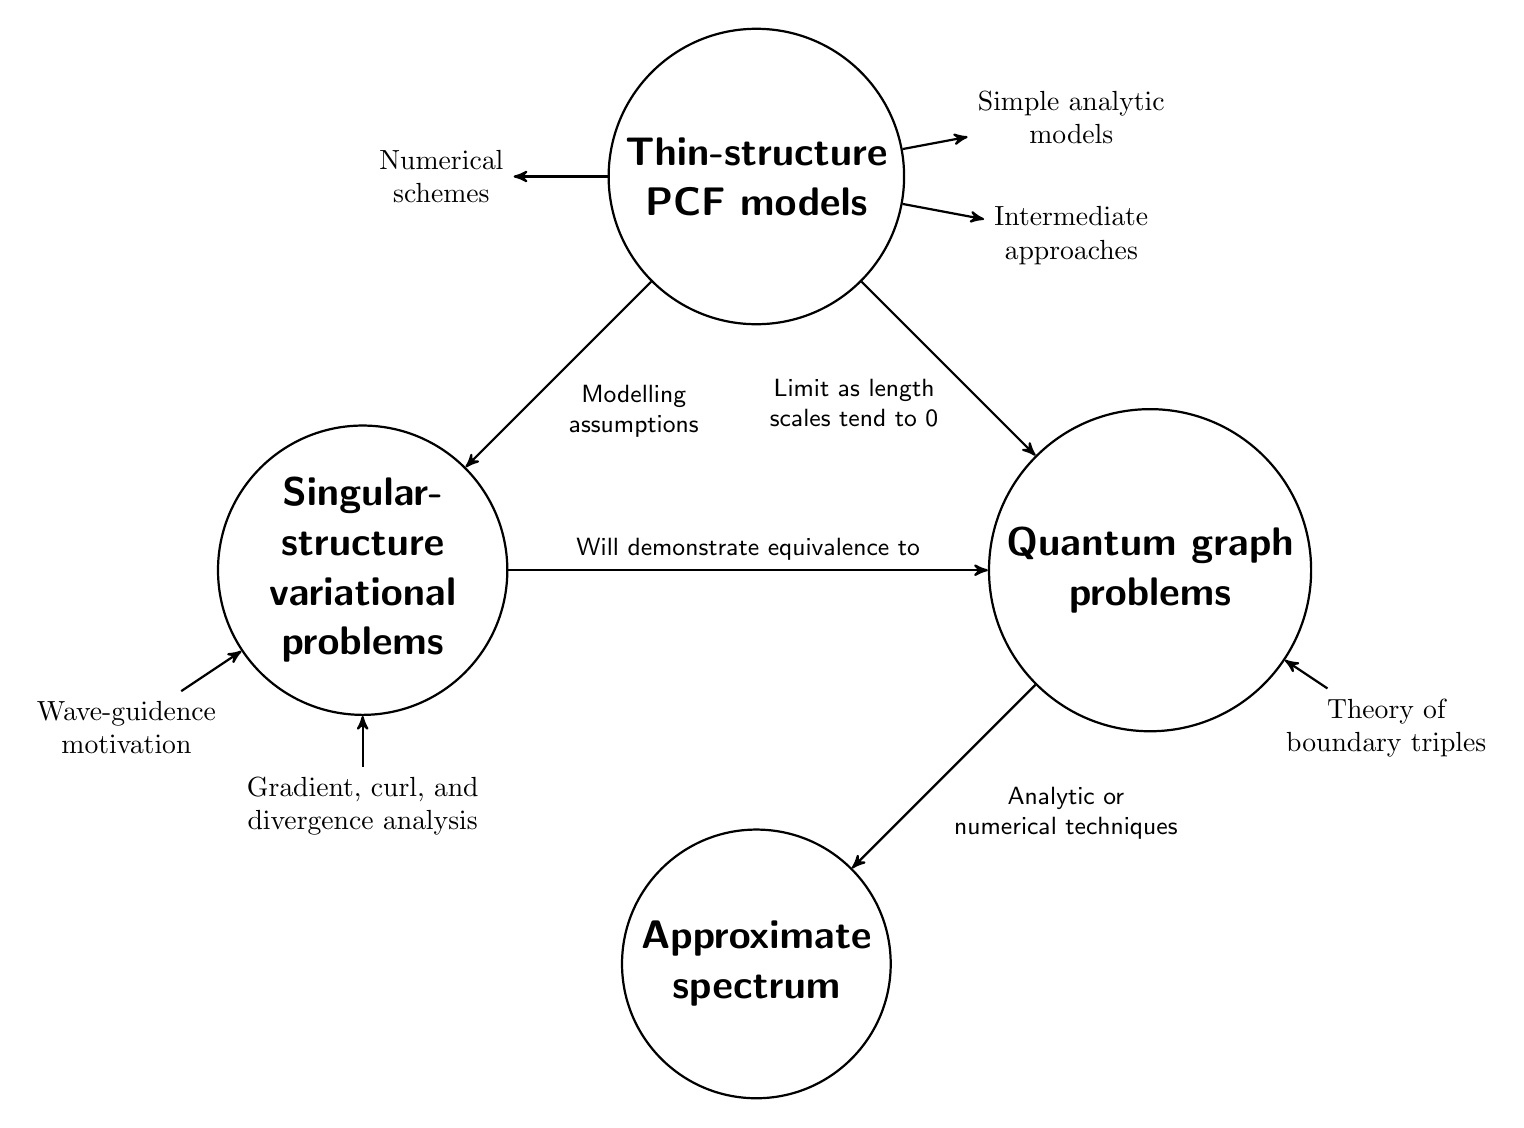
\begin{tikzpicture}[->,>=stealth',auto,node distance=3cm,thick,main node/.style={circle,draw,font=\sffamily\Large\bfseries}]

	%nodes
	\node[main node, align=center] (TS) at (0,0) {Thin-structure \\ PCF models};
	\node[main node, align=center] (SS) at (-5,-5) {Singular- \\ structure \\ variational \\ problems};
	\node[main node, align=center] (QG) at (5,-5) {Quantum graph \\ problems};
	\node[main node, align=center] (Goal) at (0,-10) {Approximate \\ spectrum};
	
	\node[align=center] (NumMod) at (-4, 0) {Numerical \\ schemes};
	\node[align=center] (ARROW) at (4, 0.75) {Simple analytic \\ models};
	\node[align=center] (Intermediate) at (4,-0.75) {Intermediate \\ approaches};
	
	\node[align=center] (GDC) at (-5,-8) {Gradient, curl, and \\ divergence analysis};
	\node[align=center] (WaveMotivation) at (-8,-7) {Wave-guidence \\ motivation};
	
	\node[align=center] (MMat) at (8,-7) {Theory of \\ boundary triples};
	
	%edges between main topics
	\path[every node/.style={font=\sffamily\small}]
		(TS) edge node[anchor=north west, align=center] {Modelling \\ assumptions} (SS)
		(SS) edge node[anchor=south] {Will demonstrate equivalence to} (QG)
		(TS) edge node[anchor=north east, align=center] {Limit as length \\ scales tend to 0} (QG)
		(QG) edge node[anchor=north west, align=center] {Analytic or \\ numerical techniques} (Goal);
		
	%arrows off TS
	\path[every node/.style={font=\sffamily\small}]
		(TS) edge (NumMod)
		(TS) edge (ARROW)
		(TS) edge (Intermediate)
	%arrows off SS
		(GDC) edge (SS)
		(WaveMotivation) edge (SS)
	%arrows off QG
		(MMat) edge (QG);


\end{tikzpicture}

\end{document}